\chapter{Risultati}
\label{chapter:Risultati}
In questo capitolo vengono presentati i risultati ottenuti. Si inizia con una panoramica dei risultati riportati nel lavoro originale, al fine di avere un riferimento di partenza, per poi illustrare i risultati sperimentali ottenuti sul nuovo dataset.
\section{EPIC-KITCHENS}
In principio AMEGO è stato valutato sul dataset EPIC-KITCHENS, confrontando le prestazioni con diverse baseline comunemente adottate nel task di video-QA:
\begin{itemize}
    \item \textbf{Semantic-free QA (SF-QA)} utilizza modelli vision-language, come CLIP \cite{radford2021learningtransferablevisualmodels}, per mappare query, video e risposte nello stesso spazio di embedding. Le feature visive vengono estratte dai frame del video, dai patch delle query e dalle risposte, mentre le feature testuali provengono dalla domanda. L'embedding della query è ottenuto come media delle feature, e la risposta con la similarità più alta viene selezionata.
    
    \item \textbf{SF-QA (obj)} è una variante di SF-QA che include anche le feature visive degli oggetti attivi rilevati da \cite{shan2020understandinghumanhandscontact}.
    
    \item \textbf{Semantic QA (S-QA)} sfrutta \emph{captioner} pre-addestrati per generare un sommario semantico del video. Si usano LaViLa \cite{zhao2022learningvideorepresentationslarge} per il video egocentrico e BLIP-2 \cite{li2023blip2bootstrappinglanguageimagepretraining} per i patch della query. Le caption vengono poi passate a LLaMA-2-7B \cite{touvron2023llama2openfoundation} per rispondere alle domande. Se il testo supera i 4096 token, viene sottocampionato.
    
    \item \textbf{Multi-round semantic QA (LLoVi)} \cite{zhang2024simplellmframeworklongrange} funziona in due round: prima sintetizza le caption del video alla luce della domanda, poi risponde alla query usando il sommario generato.
\end{itemize}

I risultati di AMEGO si dividono in: AMEGO-S e AMEGO-L, a seconda della dimensione del visual feature extractor (ViT-S/B vs ViT-L).

\begin{table}[ht]
    \centering
    \caption{Accuracy (\%) sulle diverse query di AMB. Migliori valori in grassetto.}
    \resizebox{\textwidth}{!}{%
    \begin{tabular}{|l|c|c|c|c|c|c|c|c|c|}
    \hline
    \multirow{2}{*}{\textbf{Method}} & \multicolumn{4}{c|}{\textbf{SQ}} & \multicolumn{2}{c|}{\textbf{CO}} & \multicolumn{2}{c|}{\textbf{TG}} & \multirow{2}{*}{\textbf{Total}} \\
    \cline{2-9}
    & Q1 & Q2 & Q3 & Q4 & Q5 & Q6 & Q7 & Q8 & \\
    \hline
    Random & 20.0 & 20.0 & 20.0 & 20.0 & 20.0 & 20.0 & 20.0 & 20.0 & 20.0 \\
    \hline
    SF-QA & 13.7 & 21.6 & 22.5 & 26.8 & 22.1 & 31.9 & 23.7 & 26.2 & 22.0 \\
    SF-QA (obj) & 13.1 & 23.4 & 22.6 & 23.2 & 21.7 & 26.1 & 23.8 & 25.2 & 21.2 \\
    \hline
    S-QA (LaViLa) & 20.9 & 20.6 & 21.2 & 24.6 & 24.9 & 27.1 & 21.4 & 22.6 & 22.4 \\
    S-QA (BLIP-2) & 23.9 & 22.0 & 22.5 & 23.3 & 27.5 & 27.0 & 20.2 & 24.1 & 23.6 \\
    S-QA (LaViLa+BLIP-2) & 22.8 & 22.2 & 21.4 & 22.6 & 25.1 & 26.1 & 21.4 & 24.5 & 22.9 \\
    \hline
    LLoVi (LaViLa) & 21.1 & 20.2 & 20.8 & 21.0 & 21.2 & 20.3 & 20.5 & 21.6 & 20.8 \\
    LLoVi (BLIP-2) & 22.3 & 21.4 & 21.8 & 22.2 & 25.6 & 26.7 & 18.1 & 22.2 & 22.4 \\
    LLoVi (LaViLa+BLIP-2) & 22.8 & 21.9 & 21.5 & 24.6 & 25.3 & 26.5 & 18.5 & 19.8 & 22.6 \\
    \hline
    AMEGO - S & 32.0 & 35.1 & 34.8 & 35.8 & 24.7 & 37.8 & 33.6 & 44.3 & 33.8 \\
    AMEGO - L & \textbf{33.7} & \textbf{36.3} & \textbf{37.2} & \textbf{38.3} & \textbf{27.6} & \textbf{44.3} & \textbf{34.7} & \textbf{48.9} & \textbf{36.3} \\
    \hline
    \end{tabular}%
    }
\end{table}

Tutte le baseline ottengono risultati migliori sulle query relative alla \emph{concurrency}, probabilmente perché sfruttano pattern ricorrenti presenti nei dati di addestramento, ad esempio una padella spesso utilizzata sul piano cottura \cite{goletto2024amego}. Tuttavia, le performance complessive rimangono vicine alla soglia della scelta casuale.

AMEGO invece ottiene buoni risultati su tutte le tipologie di query, superando le baseline con un margine consistente (+12.7\%). La domanda in cui AMEGO mostra maggior difficoltà è Q5, a causa dei limiti attuali dei detector di interazione mano-oggetto nel predire oggetti multipli che interagiscono contemporaneamente con la stessa mano del soggetto.

\section{ENIGMA-51}
Le valutazioni sono state effettuate sul test-set di ENIGMA-51, che comprende i seguenti video: 

\begin{center}
    \{46, 47, 49, 53, 65, 66, 85, 86, 88, 89, 95, 107, 131, 141, 143, 144\}
\end{center}

Un aspetto rilevante è che, in presenza di più oggetti con lo stesso punteggio, AMEGO seleziona quello corretto in modo casuale. 
Tale meccanismo introduce una variabilità nei risultati; per stimarne in maniera più robusta le prestazioni, 
l'esperimento è stato ripetuto per circa 100 iterazioni, calcolando i valori medi di accuracy.
In media, il modello ha raggiunto una \textbf{accuracy totale del 21.94\%}. 
Nella tabella ~\ref{table:acc_videos} viene riportata l'accuracy raggruppata per ogni video.

\begin{table}[ht]
    \centering
    \caption{Accuracy media (\%) sul test-set di enigma. Migliori valori in grassetto.}
    {\footnotesize
    \begin{tabular}{|c|c|c|} 
    \hline
    \textbf{Video ID} & \textbf{Random (\%)} & \textbf{AMEGO - L (\%)} \\
    \hline
    46  & \textbf{20} & 18.23 \\
    47  & 20.0 & \textbf{27.36} \\
    49  & 20.0 & \textbf{35.76} \\
    53  & \textbf{20} & 10.87 \\
    65  & 20.0 & \textbf{26.86} \\
    66  & \textbf{20} & 9.19 \\
    85  & 20.0 & \textbf{37.37} \\
    86  & 20.0 & \textbf{26.56} \\
    88  & 20.0 & \textbf{24.32} \\
    89  & 20.0 & \textbf{33.90} \\
    95  & 20.0 & \textbf{21.60} \\
    107 & \textbf{20} & 15.46 \\
    131 & 20.0 & \textbf{35.25} \\
    141 & \textbf{20} & 18.21 \\
    143 & \textbf{20} & 7.71 \\
    144 & 20.0 & \textbf{30.81} \\
    \hline
    \textbf{Total} & 20.0 & \textbf{23.72} \\
    \hline
    \end{tabular}%
    }
    \label{table:acc_videos}
\end{table}

Si osservano risultati non sempre soddisfacenti: in alcuni video l'accuracy scende al di sotto della soglia casuale (20\%), 
mentre in altri supera sensibilmente le prestazioni originali. 
Analizzando le percentuali per ogni domanda si evidenzia che \textbf{203} query hanno totalizzato accuracy nulla. 
Per approfondire la natura dei risultati, si analizza la query \texttt{Q5\_000089}, scelta come caso esemplificativo per evidenziare la criticità principale riscontrata.

Come si nota nella Fig.~\ref{fig:answers_zero_acc}, nonostante le patch della VQ e delle varie risposte appaiono ben distinte, il modello non seleziona mai la risposta corretta. Per comprendere tale comportamento è utile osservare la struttura della memoria di AMEGO, fornita come file JSON. Di particolare importanza sono i seguenti campi:
\begin{itemize}
    \item \texttt{track\_id}: identificativo univoco del tracklet.
    \item \texttt{obj\_bbox}: bounding box dell'oggetto
    \item \texttt{num\_frame}: lista dei frame in cui l'oggetto è rilevato durante l'interazione.
    \item \texttt{cluster}: ID d'istanza assegnato al tracklet per raggruppare interazioni simili dello stesso oggetto.
\end{itemize}

Come discusso nei capitoli precedenti, AMEGO risponde alle query valutando la presenza di \emph{overlap} temporali tra oggetti che il modello considera appartenenti allo stesso identificativo (\texttt{cluster}). Il problema può quindi risiedere nell'assegnazione delle istanze ai cluster.  

Per approfondire l'analisi, è stato utilizzato lo script di visualizzazione dei cluster discusso nel Capitolo~\ref{cap:Esperimenti}. Dall'analisi emerge che il modello di hand-object detection riesce a individuare correttamente gli oggetti a livello generale, e il \emph{tracker} mantiene buone coerenze spaziali. Tuttavia, sorge un limite significativo legato al livello di dettaglio richiesto: nelle annotazioni di ENIGMA vengono specificati particolari molto piccoli come connettori o il tipo di scheda. Come mostrato in Fig.~\ref{fig:cluster2-10}, il modello, non essendo stato addestrato su dataset industriali, tende a raggruppare in modo grossolano elementi complessi, arrivando a considerare l'intero quadro elettrico come un'unica istanza.

Un ulteriore limite emerge quando oggetti visivamente simili vengono confusi tra loro. Come mostrato in Fig.~\ref{fig:cluster24}, bastano piccole somiglianze, anche solo nel colore o nella forma, affinché il modello li raggruppi nello stesso cluster. Questo porta a difficoltà nel distinguere strumenti affini, come diversi tipi di cacciaviti, pinze o saldatori, oppure componenti che ricordano visivamente un cavo.

Questo comportamento ricorre con una certa frequenza nei cluster. Per valutare se tale fenomeno potesse effettivamente influenzare i risultati, è stata adottata una strategia di “rilassamento” delle regole di valutazione dell'accuracy, considerando come corrette anche risposte associate a oggetti visivamente molto simili. In particolare, sono state applicate le seguenti indicazioni:
\begin{itemize}
    \item \textbf{Socket}: nelle annotazioni sono presenti quattro tipologie distinte, qui considerate come un'unica categoria.
    \item \textbf{Bottoni}: unificazione di tutte le varianti.
    \item \textbf{Board}: accorpamento delle diverse tipologie di schede.
    \item \textbf{Cavi}: unificazione tra power supply, probe tips e clips.
\end{itemize}

Applicando questo rilassamento, l'accuracy raggiunge il valore di \textbf{28.86\%}, molto vicino a quello riportato nel paper originale.

\begin{figure}[ht]
    \centering
    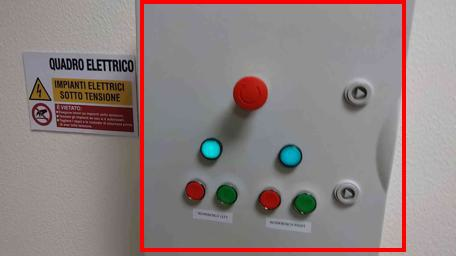
\includegraphics[width=0.5\linewidth]{Images/cluster2-10.jpg}
    \caption{HOI relativo al \texttt{cluster=2} con \texttt{track\_id = 10}.}
    \label{fig:cluster2-10}
\end{figure}

\begin{figure}[ht]
    \centering
    % Adjusted column widths to prevent overflow
    \begin{tabular}{>{\centering\arraybackslash}m{0.29\linewidth} 
                    >{\centering\arraybackslash}m{0.29\linewidth} 
                    >{\centering\arraybackslash}m{0.29\linewidth}}
        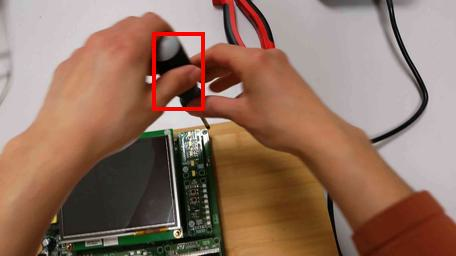
\includegraphics[width=\linewidth]{Images/cluster24-0.jpg} &
        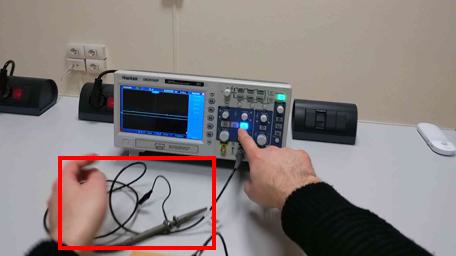
\includegraphics[width=\linewidth]{Images/cluster24-1.jpg} &
        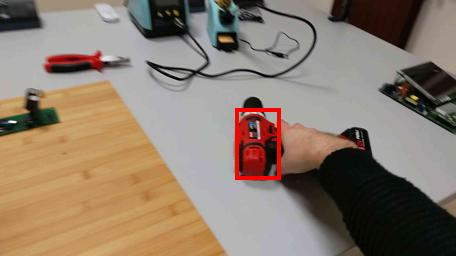
\includegraphics[width=\linewidth]{Images/cluster24-2.jpg} \\
        (a) \texttt{id=2413} & (b) \texttt{id=1138} & (c) \texttt{id=2047}
    \end{tabular}
    \caption{HOI relativi al \texttt{cluster=24}}
    \label{fig:cluster24}
\end{figure}

\begin{table}[H]
    \centering
    \caption{\raggedright VQ e risposte per la query \texttt{Q5\_000089}: per ogni classe sono mostrate tre versioni.}
    \label{fig:answers_zero_acc}
    
    \renewcommand{\arraystretch}{1.0}  % altezza riga normale
    \setlength{\tabcolsep}{3pt}        % spazio colonne

    % macro con larghezza adattata
    \newcommand{\ansimg}[1]{\includegraphics[width=0.28\linewidth,height=2.6cm,keepaspectratio]{#1}}

    % ridimensioniamo l'intera tabella per occupare la pagina
    \resizebox{\textwidth}{!}{%
    \begin{tabular}{|>{\centering\arraybackslash}m{2.0cm}|c|c|c|}
        \hline
        \textbf{Tipo} & \textbf{Versione 1} & \textbf{Versione 2} & \textbf{Versione 3} \\
        \hline
        VQ & \ansimg{Images/zeroaccvq1.jpg} & \ansimg{Images/zeroaccvq2.jpg} & \ansimg{Images/zeroaccvq3.jpg} \\
        \hline\hline
        ANS\_1 & \ansimg{Images/zero_acc_ans1-1.jpg} & \ansimg{Images/zero_acc_ans1-2.jpg} & \ansimg{Images/zero_acc_ans1-3.jpg} \\
        \hline
        ANS\_2 & \ansimg{Images/zero_acc_ans2-1.jpg} & \ansimg{Images/zero_acc_ans2-2.jpg} & \ansimg{Images/zero_acc_ans2-3.jpg} \\
        \hline
        ANS\_3 & \ansimg{Images/zero_acc_ans3-1.jpg} & \ansimg{Images/zero_acc_ans3-2.jpg} & \ansimg{Images/zero_acc_ans3-3.jpg} \\
        \hline
        ANS\_4 & \ansimg{Images/zero_acc_ans4-1.jpg} & \ansimg{Images/zero_acc_ans4-2.jpg} & \ansimg{Images/zero_acc_ans4-3.jpg} \\
        \hline
        ANS\_5 & \ansimg{Images/zero_acc_ans5-1.jpg} & \ansimg{Images/zero_acc_ans5-2.jpg} & \ansimg{Images/zero_acc_ans5-3.jpg} \\
        \hline
    \end{tabular}%
    }
\end{table}